% Define the page style
\fancypagestyle{chapterstyle}{
   \fancyhead[L]{\nouppercase{\rightmark}}
   \fancyhead[R]{Projet de fin d'études 2023-2024}
   \fancyfoot[C]{\vspace{20pt}\thepage} % Adjust the vertical space here
   \setlength{\headheight}{20pt}
   \setlength{\footskip}{30pt} % Adjust the value as needed
}

\chapter{Contexte Général}
\pagestyle{chapterstyle}
Ce chapitre met en œuvre le contexte générale du projet. Dans un premier temps, il
présente l’organisme d’accueil 4D Logiciels Maroc, son historique, sa structure, sa présence
dans le monde, ses services et son organigramme interne. Dans un deuxième temps, il décrit
la problématique, le contexte, et les objectifs derrière le développement de ce projet. Dans
un troisième temps, il détaille la conduite du projet mettant en lumière la méthodologie
suivie et la planification à l’aide du diagramme de Gant.



\newpage
\vspace{1cm}
% \section{Introduction}


%%%%%%%%%%%%%%%%%%%% SECTION 2 %%%%%%%%%%%%%%%%%%%%%%%

\section{Présentation de l’organisme d’accueil}
\subsection{Organisme d'accueil}

4D Logiciels, fondée en 1984 par Laurent Ribardière, est une entreprise pionnière dans
le domaine du développement d’applications professionnelles. Son objectif initial était de
simplifier la création d’applications pour les entreprises en utilisant une base de données
relationnelle entièrement graphique, une innovation favorisée par l’industrie logicielle.
\newline

En tant que l’un des premiers éditeurs de logiciels français, 
4D a étendu son rayonnement à l’échelle internationale, avec 
une présence sur les cinq continents et des filiales
dans cinq pays, y compris le Maroc


\begin{figure}[h]
    \centering
    
\includegraphics[scale=1]{Images/logo-4d.jpg} % Replace with the actual filename of the IBM logo image
    \caption{Logo 4D}
    \label{fig:Logo4D}
\end{figure}


\subsubsection{Fiche signalétique de 4D Logiciels}


\begin{table}[h!]
    \centering
    \begin{tabular}{|>{\raggedright\arraybackslash}m{6cm}|>{\raggedright\arraybackslash}m{6cm}|}
    \hline
    Création & 1984 \\ 
    \hline
    Forme juridique & Société à Responsabilité Limitée à Associé Unique \\ 
    \hline
    Secteur & Conseil et développement de logiciels. \\ 
    \hline
    Siège social & Le Pecq, France \\ 
    \hline
    Taille de l’entreprise & 200-500 employés \\ 
    \hline
    \end{tabular}
    \caption{Fiche signalétique de 4D Logiciels}
    \label{tab:fiche_signaletique}
\end{table}

%%%%%%%%%%%%%%%%%%%% subsection 1 %%%%%%%%%%%%%%%%%%%%%%%

\subsubsection{Histoire de 4D}
L’entreprise 4D a été fondée en 1984, marquant le début d’une ère d’innovation dans le
domaine des bases de données. En 1985, 4D a introduit le tout premier système de gestion
de base de données relationnelles graphiques, offrant ainsi aux entreprises une nouvelle
approche visuelle de la gestion des données. Deux ans plus tard, 4D a franchi une nouvelle
étape en lançant le premier système de gestion de base de données 32 bits, établissant
ainsi de nouveaux standards de performance et de puissance. En parallèle, 4D a étendu
sa présence en créant 4D Inc. dans la Silicon Valley en 1987, ainsi que 4D Deutschland,
GmbH en 1988, renforçant ainsi son engagement sur le marché international.


\begin{figure}[h]
    \centering
    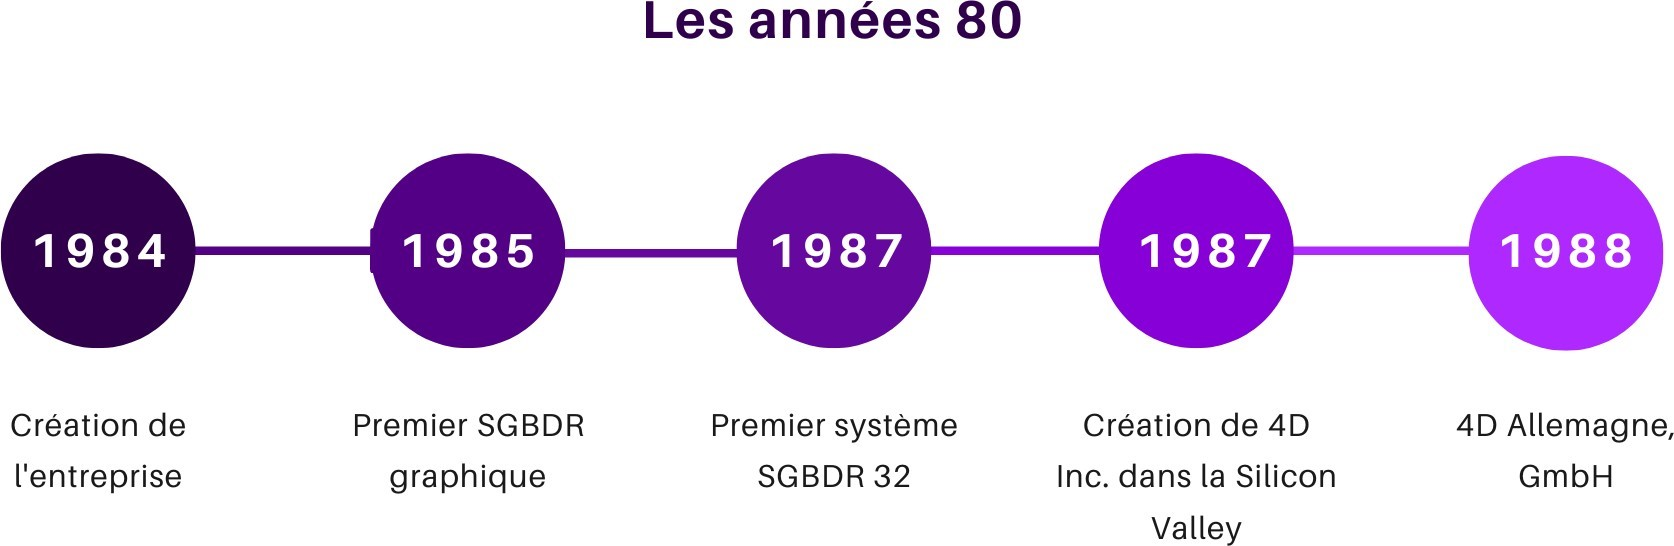
\includegraphics[scale=0.3]{Images/80.jpg} % Replace with the actual filename of the IBM logo image
    \caption{4D dans les années 80}
    \label{fig:Histoire80}
\end{figure}
\vspace{1cm}
Dans les années 90, 4D a continué d’innover en lançant en 1992 le premier système
de gestion de base de données Client/Serveur intégré. En 1995, 4D a introduit le premier
système de gestion de base de données multiplateforme, permettant aux développeurs de
créer des applications compatibles à la fois avec Mac et Windows en utilisant le même code
source. En 1997, 4D a introduit le premier système de gestion de base de données Web
dynamique, parallèlement, 4D a étendu sa présence mondiale en établissant 4D Japon en
1999, ce qui a renforcé par la suite son engagement sur le marché asiatique.

\begin{figure}[h]
    \centering
    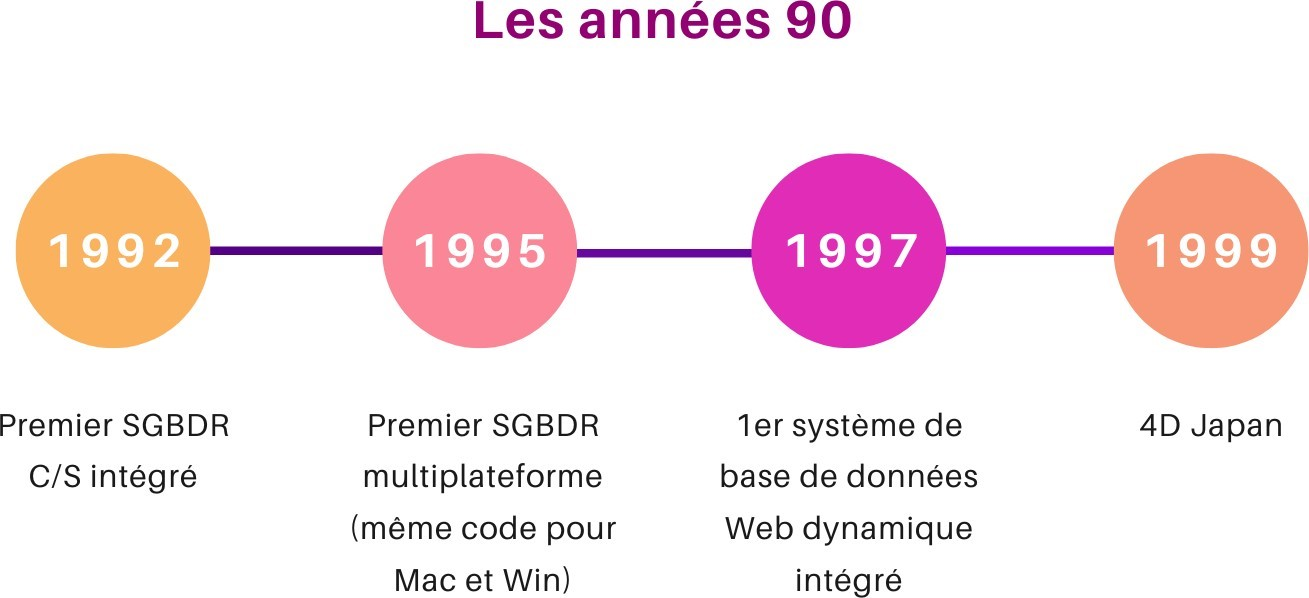
\includegraphics[scale=0.3]{Images/90.jpg} % Replace with the actual filename of the IBM logo image
    \caption{4D dans les années 90}
    \label{fig:Histoire90}
\end{figure}
% \vspace{lcm}

Ensuite, 4D Australasie Pty Ltd a été fondée en 2002, consolidant ainsi sa présence
en Australie et en Nouvelle-Zélande. En 2004, 4D a lancé la première IDE permettant de
créer des applications Client/Serveur, Web ou SOA sans avoir à modifier le code source.
En 2012, 4D a inventé la ligne de produits Wakanda, la première plateforme JavaScript de
bout en bout. En parallèle, une autre filiale a été créée au Maroc en 2012 pour renforcer
son existence sur le continent africain.
En 2016, la ligne de produits Wakanda a été reconnue par Gartner en tant que ”Cool
vendor”, confirmant ainsi l’engagement continu de 4D envers l’innovation et l’excellence
dans le domaine des technologies de développement d’applications.

\begin{figure}[h]
    \centering
    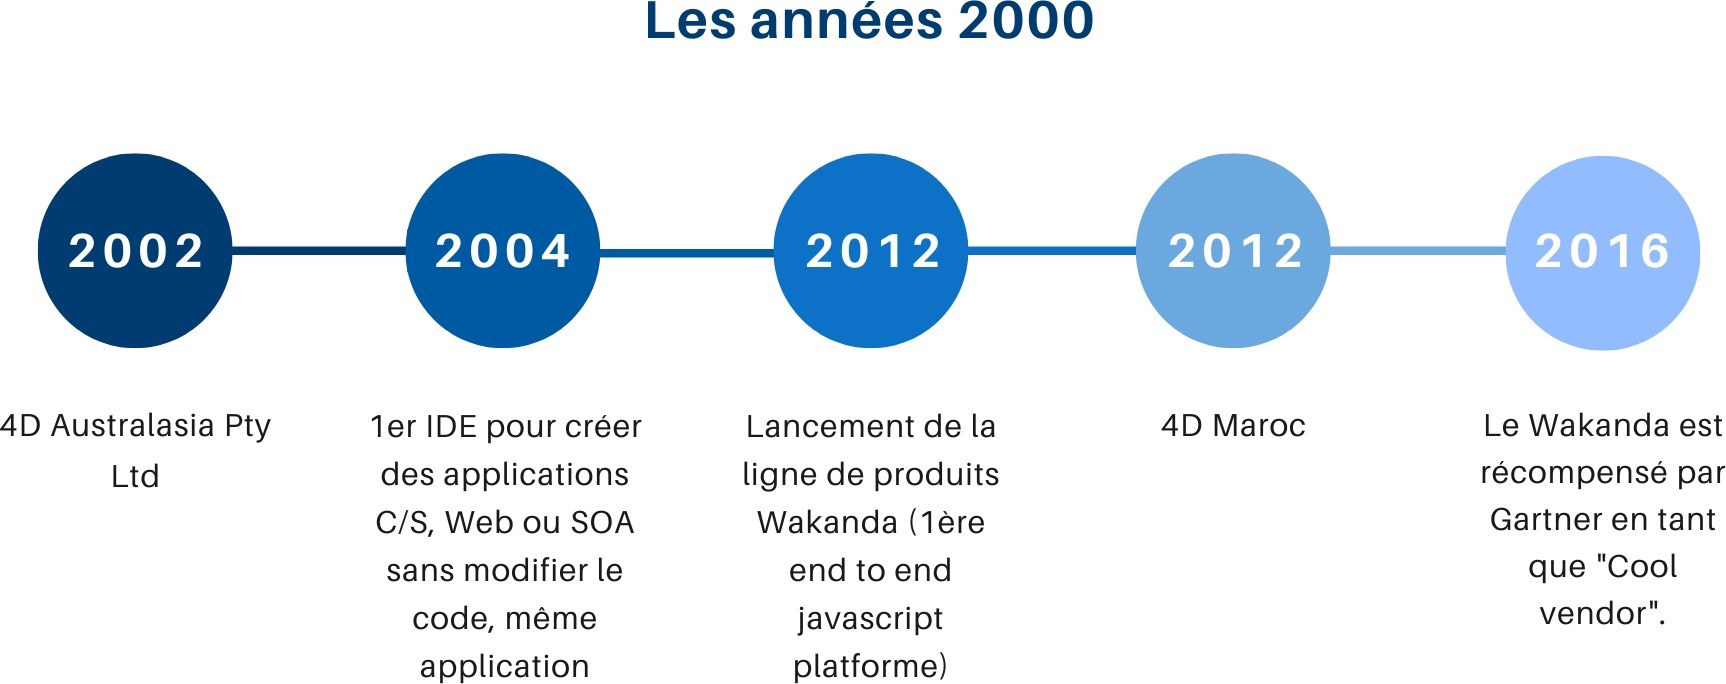
\includegraphics[scale=0.3]{Images/20.jpg} % Replace with the actual filename of the IBM logo image
    \caption{4D dans les années 2000}
    \label{fig:Histoire90}
\end{figure}


%%%%%%%%%%%%%%%%%%%% subsection 2 %%%%%%%%%%%%%%%%%%%%%%%
\vspace{3cm}
% \subsubsection{Le Langage 4D}

% 4D est une plateforme de développement productive qui permet aux clients
%  de se concentrer sur leur modèle de données et les règles 
%  et spécificités de leur métier [1].
%  Le langage 4D prend en charge l’exécution native 
%  de leur code applicatif sous macOS et Windows. 
%  4D Serveur exécute leurs applications simultanément sur les postes de travail
% / clients mobiles et sur le Web. Ils peuvent déployer des applications 
% entièrement personnalisées sous leur propre marque.
%  4D est un système de gestion de base de données 
%  relationnelle disposant d’un langage de programmation 
%  de la quatrième génération.
% \newline

% Environnement de développement intégré, 4D intègre :
% \begin{itemize}
%     \item un compilateur
%     \item un débogueur
%     \item un système de sauvegarde et de réplication
%     \item un serveur Web
%     \item un serveur et client de services web
% \end{itemize}

% \begin{figure}[h]
%     \centering
%     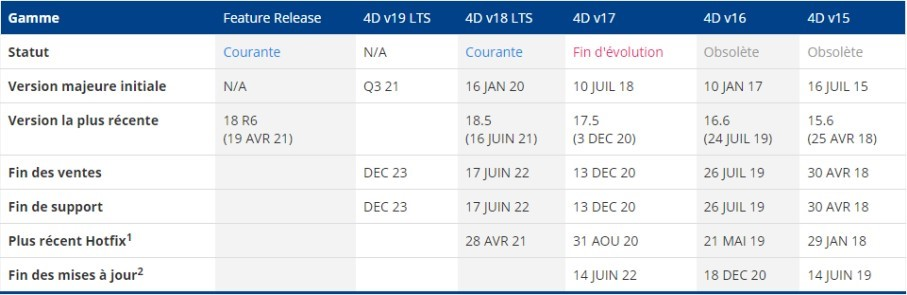
\includegraphics[scale=0.7]{Images/versions.jpg} % Replace with the actual filename of the IBM logo image
%     \caption{Anciennes versions de 4D}
%     \label{fig:AncienneVersions}
% \end{figure}

% \vspace{6cm}
% 4D v18 marque un véritable tournant dans l’histoire de 4D. Cette version propose non seulement de
% multiples nouvelles fonctionnalités, mais aussi l’amélioration de fonctions existantes. Elle introduit la gestion de version pour changer 
% la façon dont les équipes collaborent. Le format texte des bases projets permet désormais de tirer pleinement parti des systèmes de gestion de version
% (par exemple, Git, SVN, etc.). Autre fonctionnalité qui fait ses débuts dans cette nouvelle version : une solution intégrée de chiffrement des données, 
% offrant en un seul clic une sécurité maximum aux données des clients. Ces outils de chiffrement sont basés sur l’un des algorithmes les plus sûrs : 
% Advanced Encryption Standard (AES). ORDA (Object Relational Data Access), la technologie révolutionnaire d’accès et de présentation 
% des données, apporte également son lot de nouvelles fonction- nalités, telles que le Datastore distant, ouvrant de nouvelles perspectives et optimisant les 
% performances du client/serveur. Les applications métiers peuvent facilement être dé- ployées sur des appareils mobiles avec 4D for iOS, une solution 
% entièrement intégrée à 4D. De plus, 4D Write Pro, outil de PAO intégré à 4D, poursuit sa montée en puissance, le langage de programmation 4D s’enrichit et apporte de nouvelles commandes destinées à améliorer l’expérience de développement.
% \newline

% La dernière version du produit 4D, 4D v19 R8, est une version encore plus améliorée qui offre de nouvelles 
% fonctionnalités. Cette version est particulièrement intéressante pour les développeurs et les utilisateurs de 4D,
% car elle leur permet de bénéficier de performances accrues et d’une expérience utilisateur améliorée.
% En effet, les améliorations apportées à cette version ont été conçues pour répondre aux besoins des utilisateurs de manière plus efficace.
% \newline

% La version 4D v20 est actuellement en version beta, ce qui signifie 
% qu’elle est encore en phase de test. Cette version n’est pas encore 
% disponible pour une utilisation générale, mais elle est plutôt réservée 
% à un groupe restreint de testeurs qui vont l’évaluer et signaler 
% les éventuels problèmes ou bugs. Cette phase de test permet à l’équipe 
% de développement de recueillir des commentaires et des suggestions de la part 
% des testeurs afin d’améliorer la qualité du logiciel avant sa sortie officielle. 
% En bref, la version 4D v20 est en mode testing pour s’assurer qu’elle est stable et 
% fiable avant d’être rendue disponible pour le grand public.

% \vspace{0.5cm}

% \begin{figure}[h]
%     \centering
%     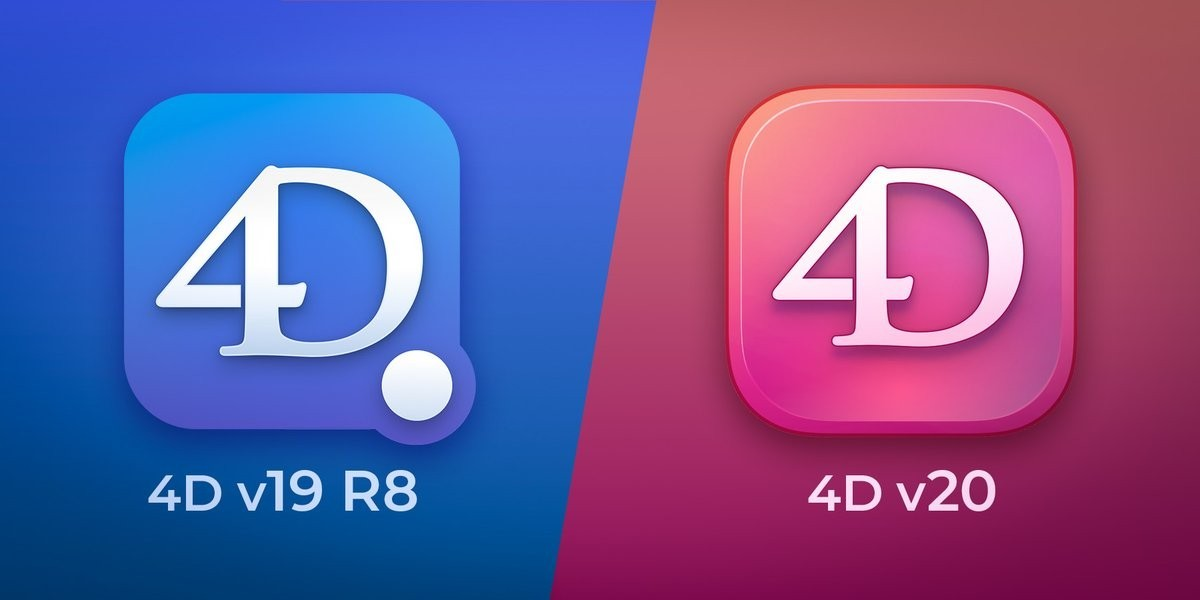
\includegraphics[scale=0.3]{Images/v19v20.jpg} % Replace with the actual filename of the IBM logo image
%     \caption{les deux nouvelles versions de 4D}
%     \label{fig:v19v20}
% \end{figure}


% %%%%%%%%%%%%%%%%%%%% subsection 3 %%%%%%%%%%%%%%%%%%%%%%%

\subsubsection{La structure du groupe 4D}
Le groupe 4D est composé d’un siège social situé en France, et de cinq filiales situées
aux États-Unis, en Allemagne, en Australie, au Japon, et au Maroc.

% \vspace{lcm}
\begin{figure}[h]
    \centering
    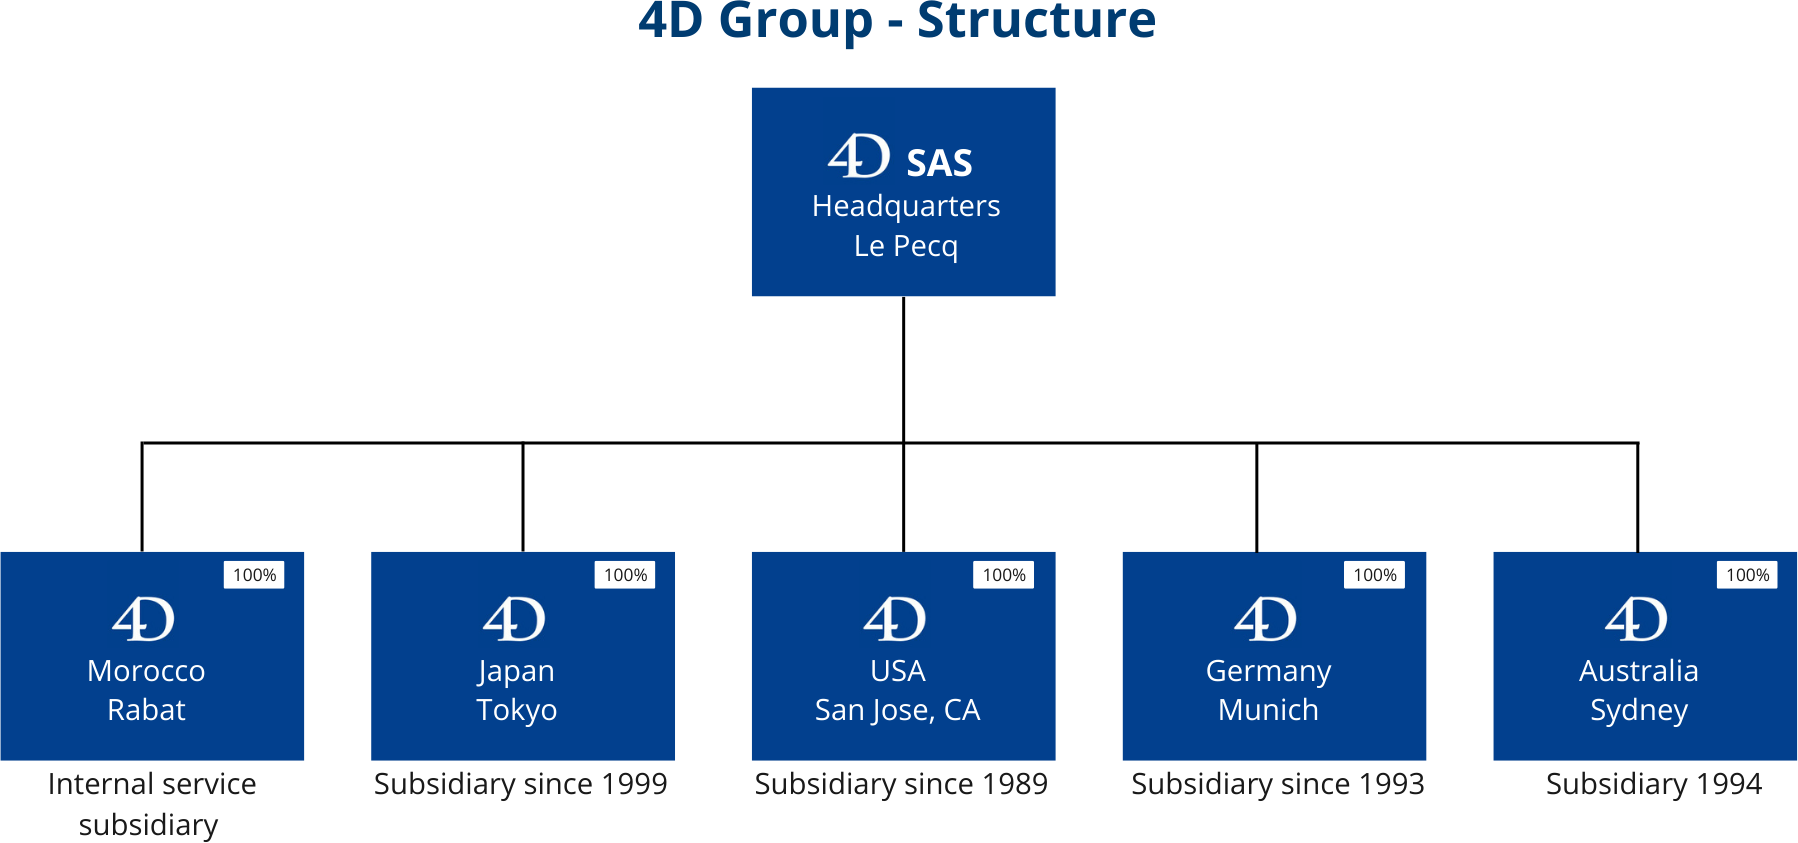
\includegraphics[scale=0.35]{Images/groupe.png} % Replace with the actual filename of the IBM logo image
    \caption{ La structure du groupe 4D}
    \label{fig:groupe}
\end{figure}

\subsubsection{Présence de 4D Logiciels dans le monde}
Comme toute société renommée, 4D recourt à ses différents partenaires pour un rendu
meilleur et un niveau d’expertise plus crédible. 4D connaît aussi une présence 
internationale grâce à ses partenaires et ses distributeurs éparpillés dans le monde, 
comme montre la figure suivante :


\begin{figure}[h]
    \centering
    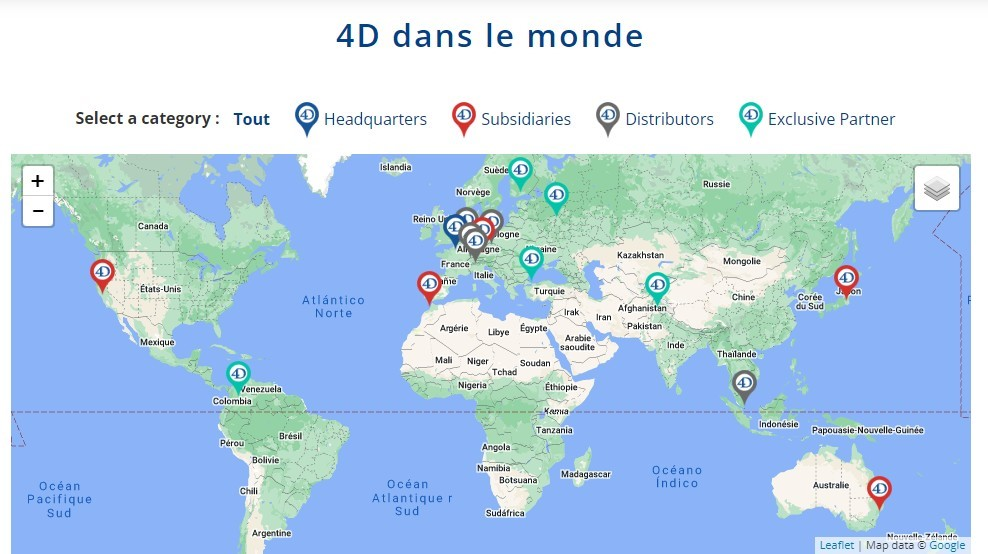
\includegraphics[scale=0.6]{Images/carte.jpg} % Replace with the actual filename of the IBM logo image
    \caption{Présence de 4D Logiciels dans le monde}
    \label{fig:carte}
\end{figure}

\vspace{3cm}

\subsubsection{Services offerts par 4D Logiciels}
4D Logiciels offre plusieurs services dans le domaine informatique, à savoir :
\\ 

\begin{itemize}
    \item  \textbf{4D Professional Services: } 4D offre une panoplie de services pour répondre aux besoins en développement logiciel, mettant à disposition une équipe qualifiée et des ressources de premier ordre à chaque étape du projet.\\
    \item \textbf{Migration des bases de données 4D :} 4D assure une transition sans heurts des bases de données 4D vers de nouveaux environnements ou versions, garantissant l’intégrité et la compatibilité des données tout en minimisant les perturbations opérationnelles.\\
    \item \textbf{ Migration 64-Bits : } 4D assure une mise à niveau efficace des applications vers des environnements 64-bits, améliorant ainsi la performance, la stabilité et la sécurité des systèmes sans compromettre la fonctionnalité existante.\\
    \item \textbf{ Développement Mobile et Web :}  4D fournit un accompagnement expert dans la conception et le développement sur mesure d’applications mobiles et web, en mettant un accent particulier sur l’optimisation de l’expérience utilisateur et l’intégration harmonieuse avec l’infrastructure informatique.\\
    \item \textbf{Audit de sécurité :}  4D réalise une évaluation approfondie de la sécurité des environnements informatiques, identifiant les vulnérabilités potentielles et proposant des stratégies proactives pour renforcer la protection des données et systèmes contre les menaces externes et internes.\\
    \item \textbf{Service Assurance Qualité et Automatisation:}  4D propose un service de tests automatisés, un service d’intégration continue ainsi qu’un service de tests fonctionnels et non fonctionnels dans l’optique d’améliorer l’efficacité des processus des applications métier de ces clients.\\
        

\end{itemize}


\subsection{Organigramme de l’organisme d’accueil}
La figure ci-dessous montre la hiéararchie de la direction générale de l’entreprise 4D
logiciels :

\begin{figure}[h]
    \centering
    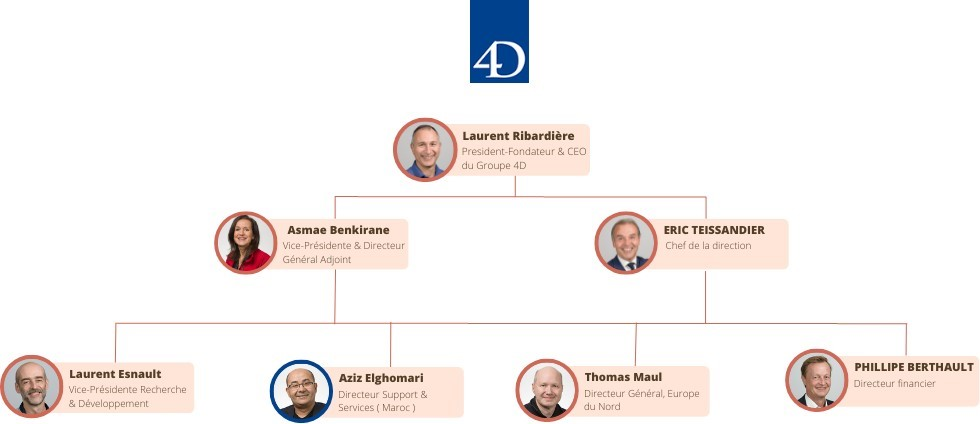
\includegraphics[scale=0.6]{Images/direction.jpg} % Replace with the actual filename of the IBM logo image
    \caption{La Direction Générale de 4D}
    \label{fig:direction}
\end{figure}


\section{Contexte général du projet}
\subsection{Cadre du projet}
Dans un environnement où la concurrence pour attirer les meilleurs talents
 est de plus en plus intense, les entreprises doivent disposer d'outils 
 efficaces pour gérer leur processus de recrutement. Actuellement, 
 4D Logiciels utilise un système disparate et manuel pour le recrutement, 
 ce qui entraîne des inefficacités et des pertes de temps. Cette situation 
 rend difficile la gestion des candidatures, la traçabilité des étapes de 
 recrutement, et la communication entre les recruteurs et les candidats.

Afin de renforcer le niveau de ses collaborateurs, 4D Logiciels souhaite 
simplifier et moderniser son processus de recrutement. L'objectif est de passer 
d'un système essentiellement manuel à une solution plus intégrée et automatisée, 
permettant d'améliorer l'efficacité, de réduire les délais de recrutement, 
et d'offrir une meilleure expérience aux candidats.

\subsection{Problématique}
L'entreprise 4D Logiciels est confrontée à une gestion inefficace
 de ses processus de recrutement, notamment lorsqu'elle publie 
 des offres d'emploi et ouvre des opportunités de stage annuelles.
4D Logiciels reçoit un grand nombre de candidatures non triées,
provenant de divers domaines, ce qui rend difficile la
sélection des candidats les plus appropriés. Les méthodes 
traditionnelles utilisées, telles que les emails, les tableurs 
et les calendriers, ne permettent pas de gérer efficacement 
ce flux de candidatures. De plus, les applications de recrutement
 disponibles sur le marché ne répondent pas pleinement aux 
 besoins spécifiques de l'entreprise en termes de processus 
 de recrutement.

En considérant les défis actuels du processus de recrutement chez
 4D Logiciels, une interrogation primordiale se profile : 
 comment transformer efficacement le processus de recrutement 
 afin de surmonter les obstacles liés au traitement manuel des 
 candidatures, à la dispersion des données et à la gestion 
 disjointe des entretiens, assurant ainsi une sélection de 
 candidats plus optimale et équitable pour l'organisation ?


\subsection{Les objectifs}

Pour répondre efficacement à la problématique identifiée,
la solution proposée doit satisfaire les objectifs suivants :

\begin{itemize}
    \item Centraliser et Automatiser la Gestion des Candidatures
    \item Améliorer la Sélection des Candidats 
    \item Optimiser la Traçabilité et la Suivi des Étapes de Recrutement 
    \item Faciliter la Communication et la Collaboration 
    \item Analyser et Optimiser les Performances du Processus de Recrutement 
    \item Offrir une Meilleure Expérience Candidat 
\end{itemize}

%%%%%%%%%%%%%%%%%%%% SECTION 4 %%%%%%%%%%%%%%%%%%%%%%%
\section{Déroulement du projet}




